\section{Phân tích Yêu cầu và Tiêu chí Thiết kế (Cơ sở Bảo Lộc)}

\subsection{Phân tích Bối cảnh và Nhu cầu}

\subsubsection{Đặc điểm Cơ sở Bảo Lộc}
Dựa trên yêu cầu của bài toán thiết kế mạng cho Cơ sở Bảo Lộc (chi nhánh của TDTU), chúng ta xác định được các đặc điểm cốt lõi sau:
\begin{itemize}
    \item \textbf{Vị trí địa lý:} Nằm xa trụ sở chính (TP.HCM), do đó yêu cầu cao về tính \textit{Sẵn sàng (Availability)} và khả năng \textit{Quản trị từ xa (Manageability)}.
    \item \textbf{Ràng buộc ngân sách:} Giới hạn ở mức 1 tỷ VNĐ cho toàn bộ thiết bị (Router, Switch, AP, Firewall). Đây là yếu tố then chốt ảnh hưởng đến việc lựa chọn thiết bị.
\end{itemize}

\subsubsection{Giả định Quy mô và Người dùng (User Requirements)}
Để việc thiết kế sát với thực tế, nhóm đưa ra các giả định về quy mô hoạt động như sau:
\begin{itemize}
    \item \textbf{Số lượng người dùng:}
    \begin{itemize}
        \item Sinh viên: 2.000 sinh viên thường xuyên.
        \item Cán bộ/Giảng viên: 100 người.
    \end{itemize}
    \item \textbf{Thiết bị đầu cuối (End-points):}
    \begin{itemize}
        \item Áp dụng chính sách BYOD (Bring Your Own Device) 100\%.
        \item Trung bình mỗi người dùng 1.2 thiết bị (Smartphone + Laptop).
        \item \textbf{Tổng tải dự kiến:} Khoảng \textbf{2.500 thiết bị} kết nối đồng thời vào giờ cao điểm.
    \end{itemize}
    \item \textbf{Ứng dụng ưu tiên:} E-learning (Moodle), Hội nghị trực tuyến (Zoom/Google Meet) kết nối về trụ sở chính.
\end{itemize}

\subsection{Xây dựng Bảng Trọng số Thiết kế (Design Matrix)}

\subsubsection{So sánh các Phương án Trọng số}
Trước khi chốt phương án cuối cùng, nhóm đã cân nhắc hai chiến lược tiếp cận khác nhau:

\begin{table}[H]
\centering
% Sử dụng tabularx với độ rộng bằng \linewidth (bề ngang trang giấy)
% Cột X cuối cùng sẽ tự động xuống dòng
\begin{tabularx}{\linewidth}{|l|c|c|X|}
\hline
\textbf{Tiêu chí} & \textbf{PA A (Kinh tế)} & \textbf{PA B (Bảo mật)} & \textbf{Nhận xét} \\ \hline
1. Kinh tế (Cost) & \textbf{30\%} & 15\% & PA A ưu tiên giá rẻ, dùng thiết bị phổ thông. \\ \hline
2. Bảo mật & 10\% & \textbf{20\%} & PA B chấp nhận chi phí cao để mua Firewall xịn. \\ \hline
3. Sẵn sàng & 15\% & \textbf{20\%} & PA B ưu tiên độ ổn định kết nối từ xa. \\ \hline
4. Hiệu suất & 20\% & 15\% & Cả hai đều đáp ứng nhu cầu cơ bản. \\ \hline
\textbf{Kết luận} & Loại bỏ & \textbf{Lựa chọn} & \textbf{Lý do:} Dữ liệu điểm thi cần bảo mật cao. \\ \hline
\end{tabularx}
\caption{So sánh giữa Phương án A (Ưu tiên Kinh tế) và Phương án B (Ưu tiên Bảo mật)}
\end{table}

\subsubsection{Bảng Trọng số Chính thức}
Dưới đây là bảng phân bổ trọng số chi tiết cho dự án theo **Phương án B**:

\begin{figure}[H]
    \centering
    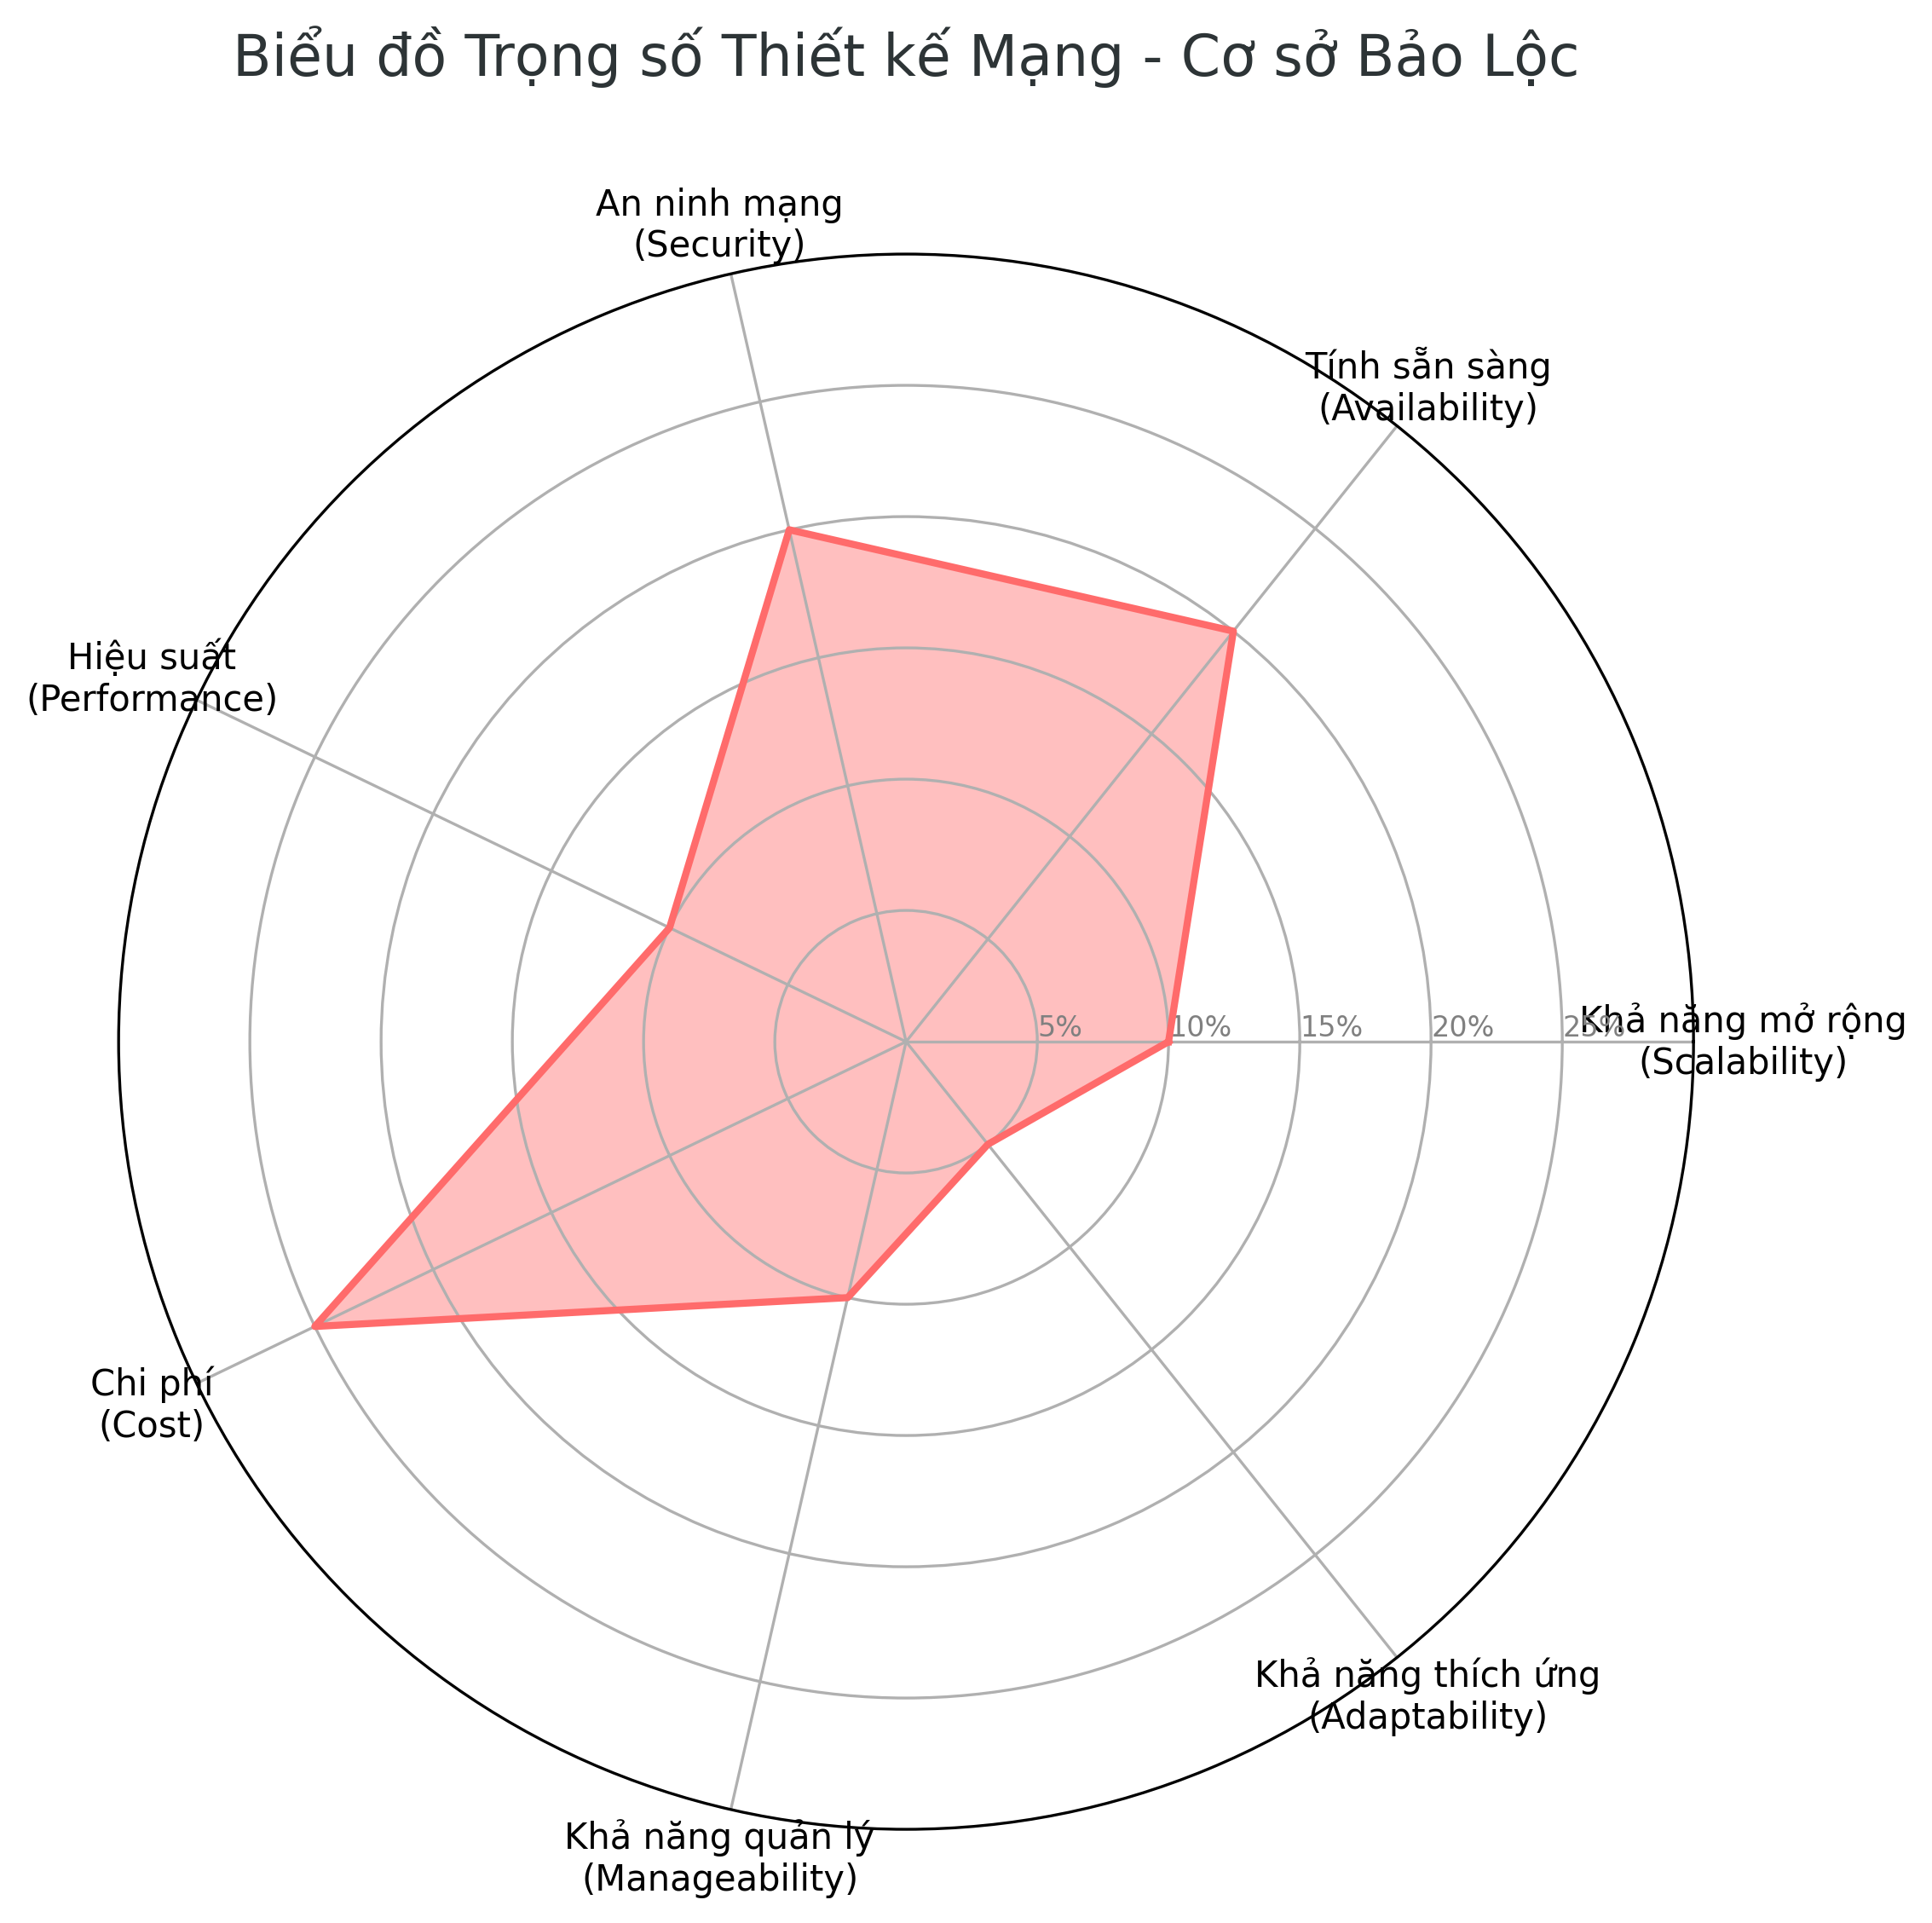
\includegraphics[width=0.7\linewidth]{image/radar_chart_analysis.png}
    \caption{Biểu đồ Radar thể hiện mức độ ưu tiên của các tiêu chí}
    \label{fig:radar_chart}
\end{figure}

\begin{table}[H]
\centering
\renewcommand{\arraystretch}{1.3}
\begin{tabularx}{\linewidth}{|c|l|c|X|}
\hline
\rowcolor[HTML]{EFEFEF} 
\textbf{STT} & \textbf{Tiêu chí (Criteria)} & \textbf{Trọng số} & \textbf{Lý giải mức độ ưu tiên} \\ \hline
1 & \textbf{An ninh (Security)} & \textbf{20\%} & \textbf{Ưu tiên cao nhất.} Bảo vệ dữ liệu điểm thi, tài chính và ngăn chặn truy cập trái phép. \\ \hline
2 & \textbf{Tính Sẵn sàng (Availability)} & \textbf{20\%} & \textbf{Ưu tiên cao nhất.} Mạng phải hoạt động 24/7. Nếu mất kết nối về trụ sở chính, việc giảng dạy bị gián đoạn. \\ \hline
3 & \textbf{Tính Kinh tế (Cost)} & \textbf{15\%} & Ngân sách 1 tỷ VNĐ là giới hạn cứng. Cần cân nhắc kỹ Cost/Performance. \\ \hline
4 & \textbf{Hiệu suất (Performance)} & 15\% & Đáp ứng tốt Web, Video Streaming. Không cần hiệu suất cực cao (như High Frequency Trading). \\ \hline
5 & \textbf{Khả năng quản lý (Manageability)} & 10\% & Cần hỗ trợ cấu hình từ xa (SSH/VPN) do đội ngũ IT tại chỗ mỏng. \\ \hline
6 & \textbf{Khả năng mở rộng (Scalability)} & 10\% & Thiết kế dư địa cho 3-5 năm tới (thêm tòa nhà, thêm sinh viên). \\ \hline
7 & \textbf{Độ trễ (Latency/Jitter)} & 5\% & Mức độ ưu tiên thấp hơn vì ít ứng dụng thoại thời gian thực (VoIP) khắt khe. \\ \hline
8 & \textbf{Khả năng thích ứng (Adaptability)} & 5\% & Sử dụng công nghệ chuẩn hóa (Ethernet/IP). \\ \hline
\end{tabularx}
\caption{Ma trận trọng số thiết kế mạng Cơ sở Bảo Lộc}
\label{tab:matrix}
\end{table}

\subsection{Phân tích sự Đánh đổi (Trade-off Analysis)}
Với ngân sách 1 tỷ VNĐ, nhóm thực hiện các quyết định đánh đổi:
\begin{itemize}
    \item \textbf{Security > Speed:} Chấp nhận độ trễ nhẹ qua Firewall để đảm bảo an toàn.
    \item \textbf{Availability > Scalability:} Dồn tiền mua Core Switch tốt thay vì mua quá nhiều cổng chờ dư thừa.
    \item \textbf{Cost-Effective Hardware:} Dùng Switch Access Ruijie để tiết kiệm chi phí cho Core Cisco/Fortinet.
\end{itemize}